\documentclass[aspectratio=169,10pt]{beamer}

%Textos en español
\usepackage[spanish]{babel}

% Document metadata
% La plantilla original usa la fuente Source Sans Pro, que no está instalada
% en este computador; se usa Lato en su lugar. Para compilar en Overleaf con
% la fuente original, reemplace estas tres líneas por:
%   \usetheme[sectionstyle=style1]{trigon}
\usetheme[sectionstyle=style1,usesourcefonts=false]{trigon}
\usepackage[T1]{fontenc}
\usepackage[default]{lato}

\setbeamerfont{title}{size=\large}

\title{Descripción y simulación de un modelo matemático para problemas acoplados fluido-estructura usando el método de elementos finitos}
\author{Sharon Nicole Acosta Caraballo}
\institute[Unicartagena]{Universidad de Cartagena \\ Programa de Matemáticas \\[2pt] \footnotesize Director: Humberto David Pérez González, PhD}
\date{\today}
% Imagen para la página del título (utilice la opción includegraphics para dimensionarla/ubicarla correctamente)
\IfFileExists{Gemini_Generated_Image_ar0dyjar0dyjar0d.png}{\titlegraphic{\includegraphics[width=\textwidth]{Gemini_Generated_Image_ar0dyjar0dyjar0d.png}}}{}

% Definir los logotipos a utilizar (comentar si no hay logotipo)
\biglogo{udc.png} % Se utiliza sólo en la portada
\smalllogo{escudo.jpg} % Se utiliza en la esquina superior derecha de los marcos normales

\usepackage{xcolor}

\definecolor{myGold}{HTML}{E79D19}
\definecolor{myBrick}{HTML}{A63C24}

\colorlet{tPrim}{myGold}
\colorlet{tSec}{myBrick}
\colorlet{tAccent}{myBrick}

% Títulos de recuadros un poco más oscuros para que se lean bien en proyector
\setbeamercolor{block title example}{fg=myGold!75!black}

% Colores auxiliares para diagramas y código (derivados de la paleta)
\colorlet{colorFluido}{myGold!20}
\colorlet{colorSolido}{gray!25}
\colorlet{colorCaja}{gray!8}

\usepackage{appendixnumberbeamer} % To use \appendix command
\pdfstringdefDisableCommands{% Fix hyperref translate warning with \appendix
\def\translate#1{#1}%
}
\usepackage{caption} % For subfigures
\usepackage{subcaption} % For subfigures
\usepackage{xspace}
\usepackage{booktabs} % Better tables
\usepackage{amsmath, amssymb}
\usepackage{tikz}
\usetikzlibrary{positioning, arrows.meta, patterns, calc, shapes.geometric}
\usepackage{pgfplots}
\pgfplotsset{compat=1.17}
\usepackage{listings}

\graphicspath{{./}{../imagenes/}}

\lstdefinestyle{FreeFEM}{
    backgroundcolor=\color{colorCaja},
    commentstyle=\color{gray},
    keywordstyle=\color{myBrick}\bfseries,
    basicstyle=\ttfamily\tiny,
    breaklines=true, showstringspaces=false, frame=single, rulecolor=\color{myBrick},
    morekeywords={solve,int2d,int1d,on}
}
\lstset{style=FreeFEM}

% Notación
\newcommand{\bu}{\mathbf{u}}
\newcommand{\bd}{\mathbf{d}}
\newcommand{\bv}{\mathbf{v}}
\newcommand{\bw}{\mathbf{w}}
\newcommand{\bz}{\mathbf{z}}
\newcommand{\bn}{\mathbf{n}}
\newcommand{\Gint}{\Gamma_{\text{int}}}

%==============================================================================
%                               COMENZAR DOCUMENTO
%==============================================================================
\begin{document}

%--------------------------------------
% Create title frame
\titleframe

%--------------------------------------
% Table of contents
%\begin{frame}{Indice}
 % \setbeamertemplate{section in toc}[sections numbered]
 % \tableofcontents[hideallsubsections]
%\end{frame} 

\begin{frame}{Objetivos}
  \begin{block}{Objetivo general}
    Describir un modelo matemático para problemas acoplados fluido-estructura utilizando el método de los elementos finitos usando FreeFEM++.
  \end{block}
  \vspace{0.3em}
  \begin{exampleblock}{Objetivos específicos}
    \begin{enumerate}
      \item Explicar los fundamentos teóricos y matemáticos del MEF, desde la formulación débil hasta su implementación numérica.
      \item Formular las ecuaciones que gobiernan el comportamiento del fluido y de la estructura.
      \item Describir el acoplamiento en la interfaz y presentar la forma débil del problema.
      \item Implementar el modelo en FreeFEM++: condiciones de frontera, parámetros físicos y esquema numérico.
    \end{enumerate}
  \end{exampleblock}
\end{frame}



\begin{frame}[allowframebreaks]{Introducción al Método de Elementos Finitos}
El \textbf{Método de los Elementos Finitos (MEF)} es una técnica numérica para aproximar soluciones de ecuaciones en derivadas parciales en dominios complejos.  
Es ampliamente utilizado en problemas multifísicos como la \textbf{interacción fluido-estructura}.  
En este trabajo se utiliza el \textbf{método de Galerkin} para modelar el flujo viscoso y el equilibrio estructural.

\vspace{0.3cm}

La aplicación del MEF se basa en tres ideas fundamentales:

\begin{itemize}
    \item \textbf{Formulación débil:} transforma el problema diferencial en una forma variacional.
    \item \textbf{Discretización del dominio:} el dominio continuo $\Omega$ se divide en una malla de elementos $\mathcal{T}_h$.
    \item \textbf{Aproximación en subespacios:} funciones base polinómicas que llevan a un sistema algebraico.
\end{itemize}

\framebreak

\textbf{Discretización del dominio:} el dominio $\Omega$ se divide en triángulos que forman la malla $\mathcal{T}_h$.

\begin{center}
    \begin{tikzpicture}[scale=0.7]
        \draw[thick] (0,0) -- (4,0) -- (4,4) -- (0,4) -- cycle;
        \draw[thick] (0,0) -- (4,4);
        \draw[thick] (2,0) -- (2,4);
        \draw[thick] (0,2) -- (4,2);
        \draw[thick] (2,2) -- (4,0);
        \draw[thick] (0,4) -- (2,2);
        \foreach \x in {0,2,4}
        \foreach \y in {0,2,4}
        \node at (\x,\y) [circle, fill, inner sep=1.5pt] {};
        \node at (2, -0.5) {Malla global $\mathcal{T}_h$};
    \end{tikzpicture}
    \hspace{1.5cm}
    \begin{tikzpicture}[scale=1.0]
        \draw[thick, fill=myGold!20] (0,0) -- (2,0) -- (1,1.732) -- cycle;
        \node at (0,0) [circle, fill, inner sep=2pt, label=below left:$z_1$] {};
        \node at (2,0) [circle, fill, inner sep=2pt, label=below right:$z_2$] {};
        \node at (1,1.732) [circle, fill, inner sep=2pt, label=above:$z_3$] {};
        \node at (1, 0.6) {$T_k$};
        \node at (1, -0.6) {Elemento triangular};
    \end{tikzpicture}
\end{center}

{\small Los elementos solo comparten vértices o aristas completas, sin nodos colgantes.}

\end{frame}

\begin{frame}{Galerkin y estimaciones de error}
  \begin{columns}[T]
    \column{0.5\textwidth}
      \begin{block}{Galerkin}
        Se busca $u_h \in V_h \subset V$ (polinomios a trozos) con
        \[
          a(u_h, v_h) = L(v_h) \quad \forall v_h \in V_h
          \;\Longrightarrow\; \mathbf{K}\mathbf{U} = \mathbf{F}.
        \]
        Ortogonalidad: $a(u-u_h, v_h) = 0$.
      \end{block}
      \begin{exampleblock}{Lema de Céa}
        \[
          \|u-u_h\|_V \le \frac{M}{\alpha}\inf_{v_h\in V_h}\|u-v_h\|_V .
        \]
      \end{exampleblock}
    \column{0.47\textwidth}
      \begin{block}{Orden de convergencia (grado $k$)}
        Si $u \in H^{k+1}(\Omega)$:
        \[
          \|u-u_h\|_{H^1} \le C\,h^{k}\,|u|_{H^{k+1}},
        \]
        y por dualidad de \textbf{Aubin-Nitsche}:
        \[
          \|u-u_h\|_{L^2} \le C\,h^{k+1}\,|u|_{H^{k+1}}.
        \]
      \end{block}
      {\small Esta teoría es la referencia para interpretar el estudio de convergencia del capítulo 3.}
  \end{columns}
\end{frame}



\begin{frame}[allowframebreaks]{El Problema Fuerte: Sistema Acoplado}
    Buscamos la terna $(\mathbf{u}, p, \mathbf{d})$ en el dominio $\Omega = \Omega_f \cup \Omega_s$:
    \vspace{0.3cm}
    
    \textbf{1. Subsistema del Fluido (Stokes) en $\Omega_f(\mathbf{d})$}
    \begin{equation*}
        \begin{cases}
            -\nabla \cdot \boldsymbol{\sigma}_f(\mathbf{u}, p) = \mathbf{0} \\
            \nabla \cdot \mathbf{u} = 0
        \end{cases}
    \end{equation*}
    Con $\boldsymbol{\sigma}_f = -p \mathbf{I} + 2\mu_f \boldsymbol{\epsilon}(\mathbf{u})$. Presenta no-linealidad geométrica al depender de $\mathbf{d}$.

    
    \vspace{0.4cm}
    \textbf{2. Subsistema de la Estructura (Elasticidad) en $\Omega_s$}
    \begin{equation*}
        -\nabla \cdot \boldsymbol{\sigma}_s(\mathbf{d}) = \mathbf{f}_v
    \end{equation*}
    Con $\boldsymbol{\sigma}_s = \lambda_s (\text{tr } \boldsymbol{\epsilon}(\mathbf{d})) \mathbf{I} + 2\mu_s \boldsymbol{\epsilon}(\mathbf{d})$ (Ley de Hooke).
\end{frame}

% ---------------- SLIDE 2 ----------------
\begin{frame}{Subsistema del Fluido (Stokes)}
    \framesubtitle{1. El Tensor de Esfuerzos ($\boldsymbol{\sigma}_f$)}
    
    Las fuerzas internas del fluido se describen con el tensor de esfuerzos:

    \vspace{0.5cm}
    \begin{equation*}
        \boldsymbol{\sigma}_f =
        \underbrace{-p\,\mathbf{I}}_{\textbf{Presión}}
        \; + \;
        \underbrace{2\mu_f\,\boldsymbol{\epsilon}(\mathbf{u})}_{\textbf{Viscosidad}}
    \end{equation*}
    \vspace{0.5cm}

    \begin{block}{Significado Físico}
        \begin{itemize}
            \item \textbf{Presión:} empuja igual en todas las direcciones.
            \item \textbf{Viscosidad:} la \textbf{fricción} entre capas del fluido al moverse.
        \end{itemize}
    \end{block}
\end{frame}

% ---------------- SLIDE 3 ----------------
\begin{frame}{Subsistema de Stokes en 2D}
    \framesubtitle{2. Equilibrio de Fuerzas y Conservación de Masa}
    
    \begin{columns}[T]
        \begin{column}{0.5\textwidth}
            \textbf{Ecuación de Momento}
            \begin{equation*}
                -\nabla \cdot \boldsymbol{\sigma}_f = \mathbf{0}
            \end{equation*}
            \begin{itemize}
                \item La presión se equilibra con la fricción viscosa.
                \item \textit{Sin inercia} ($Re \ll 1$).
            \end{itemize}
        \end{column}

        \begin{column}{0.5\textwidth}
            \textbf{Ecuación de Continuidad}
            \begin{equation*}
                \nabla \cdot \mathbf{u} = 0
            \end{equation*}
            \begin{itemize}
                \item Fluido \textbf{incompresible}: su volumen se conserva.
            \end{itemize}
        \end{column}
    \end{columns}
\end{frame}

% ---------------- SLIDE 4 ----------------
\begin{frame}{El Verdadero Reto: No-linealidad Geométrica}
    
    Todas las derivadas espaciales de las ecuaciones anteriores se calculan en el dominio del fluido $\Omega_f$.
    
    \vspace{0.5cm}
    \begin{alertblock}{La Naturaleza del Acoplamiento}
        \begin{itemize}
            \item La validez de estas componentes depende de la configuración espacial actual: \textbf{$\Omega_f(\mathbf{d})$}.
            \item El fluido genera el esfuerzo $\boldsymbol{\sigma}_f$ que deforma la estructura sólida.
            \item Al deformarse el sólido, \textbf{la frontera del fluido cambia}, alterando el espacio donde se calculan las derivadas.
        \end{itemize}
    \end{alertblock}
    
    \vspace{0.4cm}
    \begin{center}
        \textit{El fluido deforma al sólido, y el sólido modifica la pista por donde se mueve el fluido.}
    \end{center}
\end{frame}

\begin{frame}{Subsistema de la estructura (Elasticidad lineal)}
Consideremos el desplazamiento del sólido como el vector:
\[
\mathbf{d} = (d_x, d_y)
\]

El comportamiento del material depende de cómo estas componentes varían en el espacio. Esto nos lleva a tres elementos fundamentales:

\begin{block}{Flujo de análisis mecánico}
\begin{enumerate}
    \item \textbf{Cinemática:} Derivadas de $\mathbf{d} \rightarrow$ \textbf{Tensor de deformaciones}.
    \item \textbf{Constitución:} Ley de Hooke $\rightarrow$ \textbf{Tensor de esfuerzos}.
    \item \textbf{Equilibrio:} Leyes de Newton $\rightarrow$ \textbf{Ecuaciones de Navier--Lamé}.
\end{enumerate}
\end{block}
\end{frame}

% --- Deformaciones y esfuerzos (una sola diapositiva) ---
\begin{frame}{Deformaciones y esfuerzos}
  \begin{columns}[T]
    \column{0.48\textwidth}
      \begin{block}{Tensor de deformaciones}
        \[
          \boldsymbol{\epsilon}(\mathbf{d}) = \tfrac{1}{2}\left(\nabla\mathbf{d} + \nabla\mathbf{d}^T\right)
        \]
        \begin{itemize}\small
          \item $\epsilon_{xx}, \epsilon_{yy}$: \textbf{estiramiento o compresión} a lo largo de cada eje.
          \item $\epsilon_{xy}$: \textbf{cizalladura}, cambio de los ángulos rectos.
        \end{itemize}
      \end{block}
    \column{0.48\textwidth}
      \begin{block}{Ley de Hooke}
        \[
          \boldsymbol{\sigma}_s = \lambda_s (\text{tr}\,\boldsymbol{\epsilon})\,\mathbf{I} + 2\mu_s\,\boldsymbol{\epsilon}
        \]
        \begin{itemize}\small
          \item El esfuerzo es \textbf{proporcional} a la deformación.
          \item $\text{tr}\,\boldsymbol{\epsilon} = \nabla\cdot\mathbf{d}$: cambio de volumen.
        \end{itemize}
      \end{block}
  \end{columns}
\end{frame}

% --- Diapositiva 4 ---
\begin{frame}{Interpretación física de los parámetros}
Los \textbf{coeficientes de Lamé} definen la respuesta elástica:

\begin{itemize}
    \item \textbf{Primer parámetro ($\lambda_s$):} Relacionado con la resistencia a la deformación volumétrica. Controla el esfuerzo generado por cambios de volumen.
    \item \textbf{Módulo de rigidez ($\mu_s$):} Mide la resistencia al cizallamiento. 
\end{itemize}

\begin{exampleblock}{Conclusión de rigidez}
Materiales con un $\mu_s$ elevado son más rígidos frente a deformaciones laterales o torsiones, manteniendo mejor su forma angular original.
\end{exampleblock}
\end{frame}

% --- Diapositiva 5 ---
\begin{frame}{Ecuaciones de Navier--Lamé}
El equilibrio mecánico en el sólido se rige por:
\[
-\nabla \cdot \boldsymbol{\sigma}_s = \mathbf{f}_v,
\qquad
\mathbf{f}_v = (0, g)
\]

\vspace{0.3cm}
\begin{itemize}
    \item Las fuerzas internas (esfuerzos) equilibran las fuerzas externas.
    \item $\mathbf{f}_v$: \textbf{peso propio} de la viga, con $g < 0$ (hacia abajo).
\end{itemize}
\end{frame}


\begin{frame}{Condiciones en la Interfaz ($\Gamma_{\text{int}}$)}
    La interacción en $\Gamma_{\text{int}} = \partial \Omega_f \cap \partial \Omega_s$ está gobernada por tres condiciones fundamentales:
    
    \vspace{0.5cm}
    \begin{enumerate}
        \item \textbf{Compatibilidad geométrica:} 
        \[ \mathbf{x}_{\text{actual}} = \mathbf{x}_{\text{ref}} + \mathbf{d}(\mathbf{x}_{\text{ref}}) \]
        \item \textbf{Cinemática (No deslizamiento):} En estado estacionario, el fluido se detiene en la frontera del sólido.
        \[ \mathbf{u} = \mathbf{0} \]
        \item \textbf{Dinámica (Acción y reacción):} Continuidad de tracciones.
        \[ \boldsymbol{\sigma}_f \, \mathbf{n}_f + \boldsymbol{\sigma}_s \, \mathbf{n}_s = \mathbf{0}, \qquad \mathbf{n}_f = -\mathbf{n}_s \]
    \end{enumerate}
\end{frame}

\begin{frame}{Geometría y Normales}
    \begin{figure}[h!]
        \centering
        \begin{tikzpicture}[scale=1.15]
            % Dominio Fluido
            \fill[blue!10] (0,2) rectangle (4,4);
            \draw[thick] (0,2) -- (0,4) -- (4,4) -- (4,2);
            \node at (2,3) {$\Omega_f$ (Fluido)};
            
            % Dominio Sólido
            \fill[gray!20] (0,0) rectangle (4,2);
            \draw[thick] (0,0) -- (4,0) -- (4,2) -- (0,2) -- cycle;
            \node at (2,1) {$\Omega_s$ (Sólido)};
            
            % Interfaz
            \draw[ultra thick, blue] (0,2) -- (4,2);
            \node at (4.4, 2) {$\Gamma_{\text{int}}$};
            
            % Vectores normales
            \draw[->, thick, red] (2.5, 2) -- (2.5, 1.4) node[right, font=\small] {$\mathbf{n}_f$};
            \draw[->, thick, teal] (1.5, 2) -- (1.5, 2.6) node[right, font=\small] {$\mathbf{n}_s$};
            
            % Etiquetas de frontera
            \node at (-0.5, 3) {$\Gamma_{f,D}$};
            \node at (-0.5, 1) {$\Gamma_{s,D}$};
        \end{tikzpicture}
    \end{figure}
    \begin{center}
        Notar que por compatibilidad geométrica: $\mathbf{n}_f = - \mathbf{n}_s$
    \end{center}
\end{frame}

\begin{frame}{Espacios Funcionales (Bases de la Formulación)}
    Para pasar a la forma variacional, definimos los espacios de Sobolev:

    \textbf{Para el Fluido:}
    \begin{align*}
        \mathbf{V}_f &= \{ \mathbf{v} \in [H^1(\Omega_f)]^2 : \mathbf{v} = \mathbf{0} \text{ en } \Gamma_{f,D} \cup \Gamma_{\text{int}} \} \\
        Q_f &= \left\{ q \in L^2(\Omega_f) : \int_{\Omega_f} q = 0 \right\}
    \end{align*}
    
    \textbf{Para la Estructura:}
    \begin{align*}
        \mathbf{V}_s &= \{ \mathbf{w} \in [H^1(\Omega_s)]^2 : \mathbf{w} = \mathbf{0} \text{ en } \Gamma_{s,D} \}
    \end{align*}

    {\small\textit{Las funciones de prueba son nulas en las fronteras de Dirichlet. En el esquema particionado, $\mathbf{v}$ también se anula sobre $\Gamma_{\text{int}}$, donde la velocidad del fluido es un dato impuesto.}\par}
\end{frame}

\begin{frame}[allowframebreaks]{Formulación Variacional (Forma Débil)}
    Multiplicando por las funciones de prueba $(\mathbf{v}, q, \mathbf{w})$ e integrando por partes:
    
    \vspace{0.2cm}
    \textbf{Ecuación del Fluido:}
    \small
    \begin{equation*}
        \int_{\Omega_f} 2\mu_f \boldsymbol{\epsilon}(\mathbf{u}) : \boldsymbol{\epsilon}(\mathbf{v}) - \int_{\Omega_f} p (\nabla \cdot \mathbf{v}) + \int_{\Omega_f} q (\nabla \cdot \mathbf{u}) = 0
    \end{equation*}
    \normalsize
    
    \vspace{0.2cm}
    \textbf{Ecuación del Sólido:}
    \small
    \begin{equation*}
        \int_{\Omega_s} \left[ \lambda_s (\nabla \cdot \mathbf{d})(\nabla \cdot \mathbf{w}) + 2\mu_s \boldsymbol{\epsilon}(\mathbf{d}) : \boldsymbol{\epsilon}(\mathbf{w}) \right] = \int_{\Omega_s} \mathbf{f}_s \cdot \mathbf{w} + \int_{\Gamma_{\text{int}}} \mathbf{t}_s \cdot \mathbf{w}
    \end{equation*}
    \normalsize
    
    \vspace{0.3cm}
    Como $\mathbf{v} \in \mathbf{V}_f$ se anula en $\Gamma_{\text{int}}$, la integral de tracción del fluido \textbf{es cero}: la tracción $\mathbf{t}_f$ se recupera después y se transfiere al sólido como condición de Neumann ($\mathbf{t}_s$).
\end{frame}

\begin{frame}[allowframebreaks]{El Acoplamiento Global}
    En la formulación \textbf{monolítica} se usa un único espacio de prueba global:
    \begin{equation*}
        \mathbf{Z} = \left\{ \mathbf{z} \in [H^1(\Omega)]^2 : \mathbf{z} = \mathbf{0} \text{ en } \Gamma_{f,D} \cup \Gamma_{s,D} \right\},
    \end{equation*}
    cuyas funciones son \textbf{continuas y libres} sobre $\Gamma_{\text{int}}$. Con acción y reacción ($\mathbf{t}_s = -\mathbf{t}_f$) y tomando $\mathbf{v} = \mathbf{w} = \mathbf{z}$:
    
    \begin{equation*}
        \int_{\Gamma_{\text{int}}} \mathbf{t}_f \cdot \mathbf{z} \, d\Gamma + \int_{\Gamma_{\text{int}}} \mathbf{t}_s \cdot \mathbf{z} \, d\Gamma = \int_{\Gamma_{\text{int}}} (\mathbf{t}_f - \mathbf{t}_f) \cdot \mathbf{z} \, d\Gamma = 0
    \end{equation*}

    \vspace{0.5cm}
    {\small El esquema que se implementa es el \textbf{particionado}.}
\end{frame}

\begin{frame}[allowframebreaks]{Estrategia de Solución: Método Particionado}
    Debido al mal condicionamiento del sistema monolítico, usamos el algoritmo de \textbf{Dirichlet-Neumann} con relajación $\omega$:
    
    \vspace{0.3cm}
    \begin{enumerate}
        \item Resolver Fluido (Stokes) en la malla actual.
        \item Calcular la tracción del fluido (proyección $L^2$ de $\boldsymbol{\sigma}_f$).
        \item Resolver Sólido (Elasticidad) con la carga $\alpha\,\boldsymbol{\sigma}_f\bn_s$ (Neumann).
        \item Relajar desplazamiento: $\mathbf{d}_{\text{int}}^{k+1} = \omega \tilde{\mathbf{d}}^{k+1} + (1-\omega) \mathbf{d}_{\text{int}}^k$, con $\omega = 0.5$ constante (converge en 21 iteraciones; sin relajación, en 5 a 7).
        \item Actualizar malla del fluido (ALE) imponiendo $\mathbf{d}_{\text{int}}^{k+1}$ (Dirichlet).
        \item Repetir hasta que $\|\mathbf{d}_{\text{int}}^{k+1} - \mathbf{d}_{\text{int}}^k\| / \|\mathbf{d}_{\text{int}}^{k+1}\| < 10^{-6}$.
    \end{enumerate}
\end{frame}

\begin{frame}{Flujo del Algoritmo}
    \begin{figure}[h!]
        \centering
        % AJUSTE CLAVE: Limitamos el alto al 80% de la diapositiva en vez de limitar el ancho
        \resizebox{!}{0.72\textheight}{
        \begin{tikzpicture}[
            % AJUSTE CLAVE: Reducimos la distancia vertical a 0.5cm
            node distance=0.5cm and 1.5cm,
            auto,
            block/.style={rectangle, draw, fill=blue!10, text width=8em, text centered, rounded corners, minimum height=2.5em},
            decision/.style={diamond, draw, fill=green!10, text width=5em, text centered, inner sep=0pt},
            line/.style={draw, -{Latex[length=3mm]}, thick},
            cloud/.style={draw, ellipse, fill=gray!20, node distance=2cm, minimum height=2em}
            ]
            
            \node [cloud] (start) {Inicio: $\Omega_f^0, \Omega_s^0$};
            \node [block, below=of start] (fluid) {Solver Fluido (Stokes)};
            \node [block, below=of fluid] (force) {Tracción $\boldsymbol{\sigma}_f\bn_s$};
            \node [block, below=of force] (solid) {Solver Sólido};
            \node [block, below=of solid] (relax) {Relajación $\omega$};
            \node [decision, below=of relax] (check) {¿Converge?};
            \node [block, left=of force] (update) {Mover Malla (ALE)};
            \node [cloud, right=of check, node distance=2.5cm] (stop) {Fin};
            
            \path [line] (start) -- (fluid);
            \path [line] (fluid) -- (force);
            \path [line] (force) -- (solid);
            \path [line] (solid) -- (relax);
            \path [line] (relax) -- (check);
            \path [line] (check) -- node [above] {Sí} (stop);
            \path [line] (check.west) -| node [near start, above] {No} (update.south);
            \path [line] (update.north) |- (fluid.west);
        \end{tikzpicture}
        }
    \end{figure}
\end{frame}

\begin{frame}{Caso de estudio: cavidad con tapa elástica}
  \begin{columns}[T]
    \column{0.44\textwidth}
      \centering
      \begin{tikzpicture}[scale=0.62, >=stealth]
        \def\L{4} \def\H{4} \def\Es{0.5}
        \fill[blue!10] (0,0) rectangle (\L,\H);
        \node at (\L/2, \H/2) {$\Omega_f$};
        \draw[->, blue!40, thick] (\L/2+0.5, \H/2) arc (0:330:0.5);
        \draw[line width=1.2pt] (0,\H) -- (0,0) -- (\L,0) -- (\L,\H);
        \fill[pattern=north east lines] (\L,0) rectangle (\L+0.2,\H);
        \fill[pattern=north east lines] (-0.2,-0.2) rectangle (\L+0.2,0);
        \draw[fill=gray!30, draw=black, thick] (0,\H) rectangle (\L,\H+\Es);
        \node at (\L/2, \H+\Es/2) {\footnotesize $\Omega_s$};
        \draw[red, line width=1.6pt] (0,\H) -- (\L,\H);
        \foreach \y in {0.3, 1.2, 2.1, 3.0} { \draw[->, very thick, orange!80!black] (0.16,\y) -- (0.16,\y+0.6); }
        \node[orange!80!black, rotate=90, font=\scriptsize] at (-0.55,\H/2) {$\bu=(0,U_0)$};
        \node[right, font=\scriptsize] at (\L+0.2,\H/2) {$\bu=\mathbf{0}$};
        \node[below, font=\scriptsize] at (\L/2,-0.2) {$\bu=\mathbf{0}$};
        \node[red, above right, font=\scriptsize] at (\L, \H-0.45) {$\Gint$};
      \end{tikzpicture}

      \vspace{0.2em}
      {\scriptsize Cavidad $10\times10$; viga $10\times2$ empotrada en sus extremos. El fluido se mueve por la \textbf{pared izquierda}; en $\Gint$, $\bu = \mathbf{0}$.}
    \column{0.53\textwidth}
      \centering
      \footnotesize
      \begin{tabular}{lcc}
        \toprule
        \textbf{Parámetro} & \textbf{Símbolo} & \textbf{Valor} \\
        \midrule
        Módulo de Young & $E$ & 21.5 \\
        Coeficiente de Poisson & $\nu$ & 0.29 \\
        Fuerza másica & $g$ & $-0.05$ \\
        Viscosidad & $\mu_f$ & 1.0 \\
        Velocidad de pared & $U_0$ & 1.0 \\
        Intensidad de acoplamiento & $\alpha$ & 0.2 \\
        \bottomrule
      \end{tabular}

      \vspace{0.5em}
      \begin{block}{Origen del caso}
        \footnotesize Geometría y parámetros: ejemplo oficial de la documentación de FreeFEM++ (Hecht). El programa es una \textbf{implementación propia} del esquema del Capítulo 2 (Anexo A). $\alpha = 0.2$ limita la carga transmitida: \textbf{régimen de acoplamiento débil}.
      \end{block}
  \end{columns}
\end{frame}
\begin{frame}[fragile]{Discretización y transferencia de carga}
  \begin{columns}[T]
    \column{0.38\textwidth}
      \begin{block}{Espacios de elementos finitos}
        \begin{itemize}
          \item Fluido: \textbf{Taylor-Hood} $P_2/P_1$, par estable (cumple inf-sup).
          \item Sólido: $P_1$ vectorial.
        \end{itemize}
      \end{block}
    \column{0.6\textwidth}
\begin{lstlisting}[basicstyle=\ttfamily\tiny]
// Elasticidad con acoplamiento FSI
solve Elasticity([dt1,dt2],[w,s])
  = int2d(th)( lambda*div(w,s)*div(dt1,dt2)
             + 2*mus*(epsilon(w,s)'*epsilon(dt1,dt2)) )
  + int2d(th)( -gravity*s )               // peso propio
  + int1d(th,bottombeam)( -coefalpha*(    // Gamma_int
        (s11r*N.x + s12r*N.y)*w           // sigma_f: proyeccion L2
      + (s12r*N.x + s22r*N.y)*s ) )
  + on(2, 4, dt1=0, dt2=0);               // empotramiento
// Relajacion
d1[] = omega*dt1[] + (1-omega)*d1old[];
\end{lstlisting}
  \end{columns}
\end{frame}
\begin{frame}{Movimiento de malla: técnica ALE}
  \framesubtitle{ALE: \textit{Arbitrary Lagrangian-Eulerian} (Arbitraria Lagrangiana-Euleriana)}
  \vspace{0.4cm}
  Cuando la viga se deforma, la frontera del fluido cambia y la malla debe adaptarse. La técnica \textbf{ALE} mueve la malla del fluido de modo que \textbf{sus nodos de borde siguen a la viga} y los \textbf{nodos interiores se acomodan suavemente}. No es Lagrangiana pura (la malla se enredaría con el fluido) ni Euleriana pura (no podría seguir a la viga), y \textbf{conserva la topología}: los mismos triángulos, conectados igual, sin elementos invertidos ($J_K > 0$).
\end{frame}
\begin{frame}{Campos de velocidad y presión}
  \begin{columns}[c]
    \column{0.48\textwidth}
      \centering
      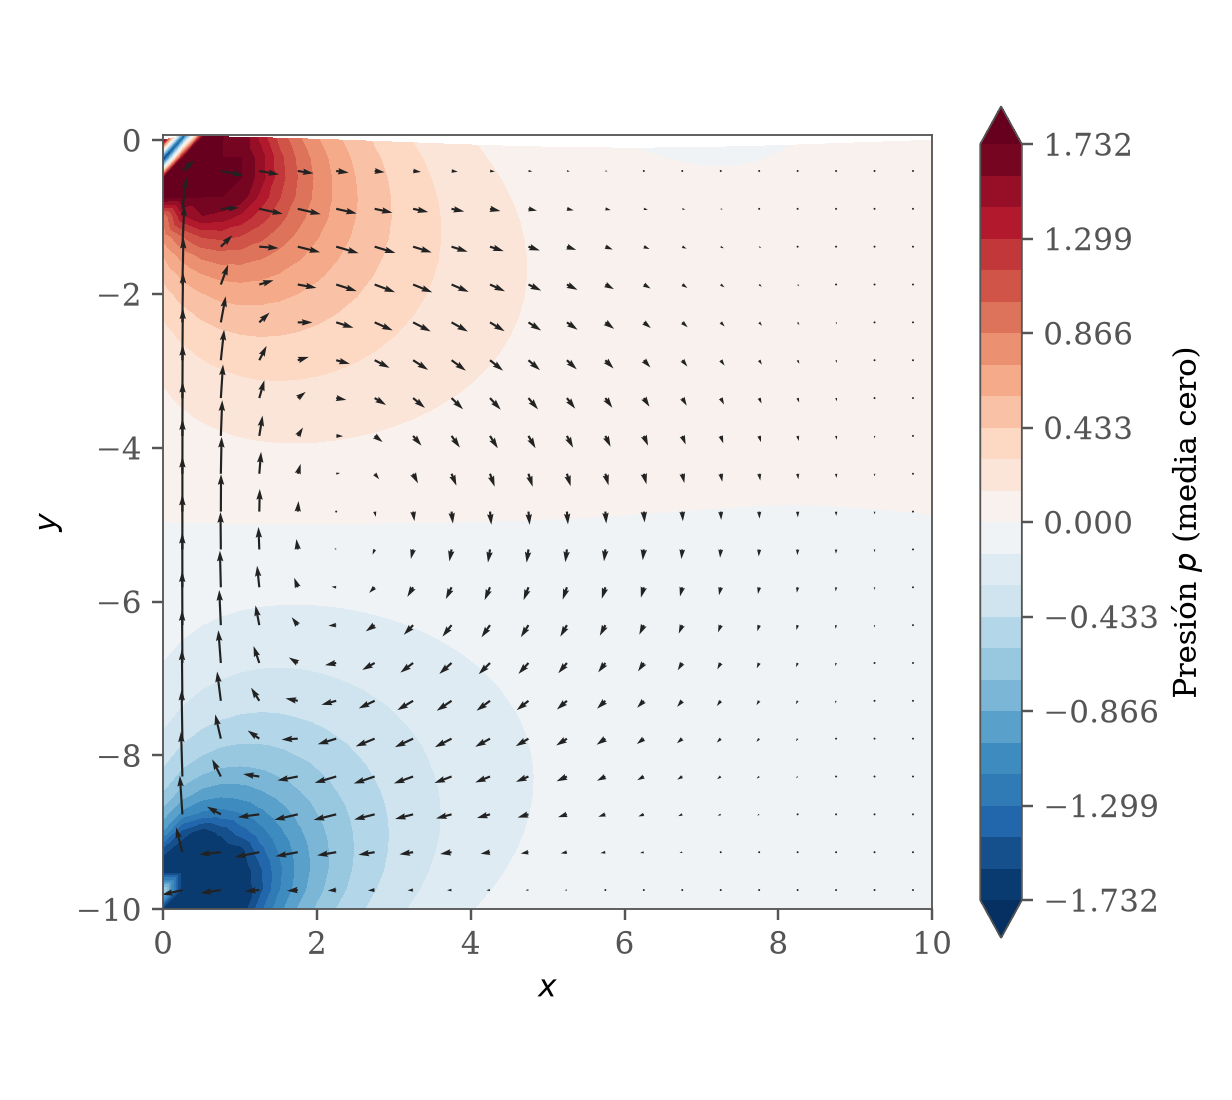
\includegraphics[height=0.66\textheight]{FSI_velocidad_presion.png}

      {\scriptsize Simulación propia, malla $N=40$.}
    \column{0.49\textwidth}
      \begin{itemize}
        \item La pared izquierda sube y arrastra el fluido: \textbf{recirculación} en la mitad izquierda.
        \item Presión \textbf{positiva arriba} y \textbf{negativa abajo}.
        \item Valores extremos en las \textbf{esquinas de la pared impulsora}: la presión es singular.
      \end{itemize}
  \end{columns}
\end{frame}
\begin{frame}{Respuesta estructural y malla deformada}
  \begin{columns}[T]
    \column{0.49\textwidth}
      \centering
      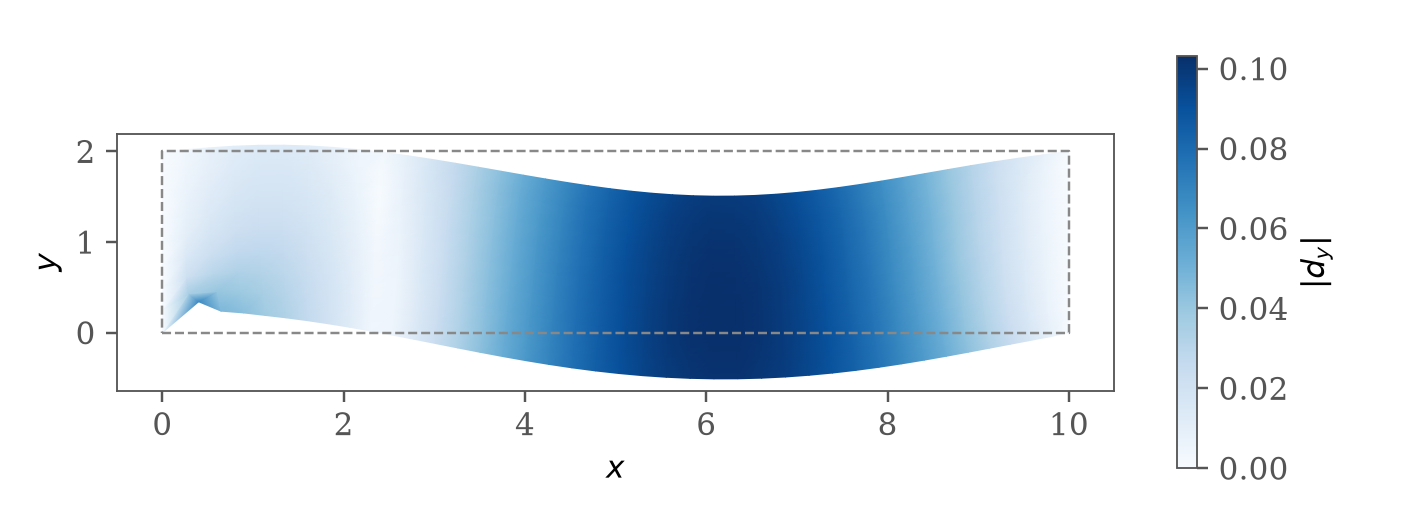
\includegraphics[width=\linewidth]{FSI_desplazamiento_viga.png}

      {\scriptsize Desplazamiento de la viga (amplificado $\times 5$).}
      \vspace{0.4em}
      \begin{itemize}\footnotesize
        \item La presión del fluido \textbf{empuja hacia arriba} y alivia el lado izquierdo.
        \item Elástica asimétrica: máximo $|d_y| \approx 0.103$ en $x\approx6$.
        \item Junto a la esquina, deformación local por la singularidad.
      \end{itemize}
    \column{0.49\textwidth}
      \centering
      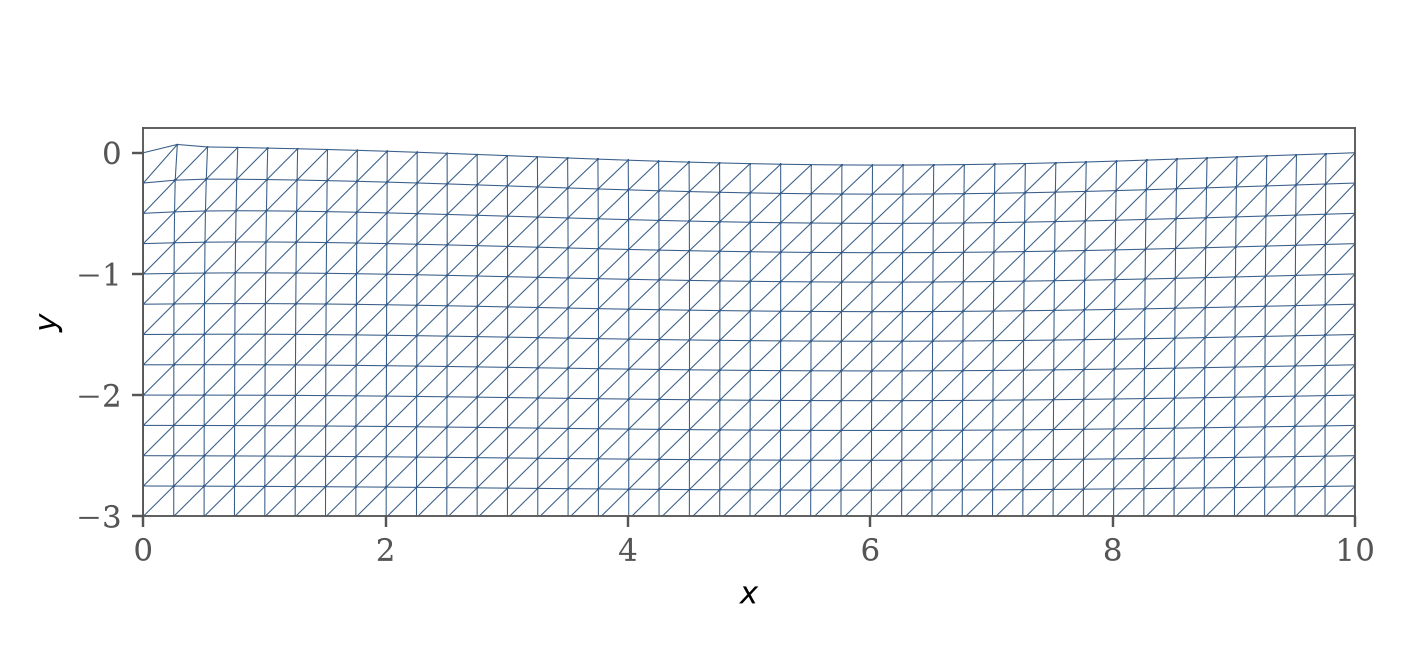
\includegraphics[width=\linewidth, height=0.36\textheight, keepaspectratio]{FSI_malla_deformada.png}

      {\scriptsize Malla deformada cerca de $\Gint$.}
      \vspace{0.4em}
      \begin{itemize}\footnotesize
        \item Nodos redistribuidos suavemente.
        \item $J_K>0$ \textbf{comprobado en todo el dominio}: cociente mínimo de áreas $0.945$ ($N=120$).
      \end{itemize}
  \end{columns}
  \vspace{0.2em}
  \centering{\scriptsize Figuras: simulación propia (Anexo A de la tesis), malla $N=40$.}
\end{frame}
\begin{frame}{Estudio de convergencia de malla}
  \begin{columns}[T]
    \column{0.47\textwidth}
      \small
      Referencia sobre-refinada ($N=120$). Error relativo de la velocidad:
      \[
        E_N = \frac{\|\bu_N - \mathcal{I}_N\bu_{\text{ref}}\|_{L^2}}{\|\mathcal{I}_N\bu_{\text{ref}}\|_{L^2}},
        \quad
        q = \frac{\log(E_{N-1}/E_N)}{\log(h_{N-1}/h_N)}
      \]
      \centering
      \footnotesize
      \begin{tabular}{cccc}
        \toprule
        $N$ & $h/L$ & $E_N$ & $q$ \\
        \midrule
        10 & $1.00\times10^{-1}$ & $8.806\times10^{-2}$ & -- \\
        20 & $5.00\times10^{-2}$ & $4.408\times10^{-2}$ & 1.00 \\
        40 & $2.50\times10^{-2}$ & $2.167\times10^{-2}$ & 1.02 \\
        80 & $1.25\times10^{-2}$ & $1.140\times10^{-2}$ & 0.93 \\
        \bottomrule
      \end{tabular}
    \column{0.5\textwidth}
      \centering
      \begin{tikzpicture}
        \begin{loglogaxis}[
            width=6.6cm, height=5.0cm,
            xlabel={$h/L$}, ylabel={$E_N$},
            grid=both, grid style={line width=.1pt, draw=gray!20},
            legend pos=north west, legend style={font=\scriptsize},
            tick label style={font=\scriptsize}, label style={font=\footnotesize}]
          \addplot+[mark=square*, line width=1.1pt, mark size=2pt, color=myBrick]
            coordinates {(0.1,0.08806) (0.05,0.04408) (0.025,0.02167) (0.0125,0.01140)};
          \addlegendentry{Simulación}
          \addplot[color=red!70!black, dashed, line width=0.9pt, domain=0.01:0.12] {0.88*x};
          \addlegendentry{$O(h)$}
        \end{loglogaxis}
      \end{tikzpicture}
  \end{columns}
  \vspace{0.2em}
  \begin{block}{Lectura}
    \small Al dividir $h$ a la mitad el error baja $\approx 2$ veces: la tasa experimental es \textbf{aproximadamente lineal}. La deflexión máxima se estabiliza (cambia $<1\%$ entre $N=80$ y la referencia).
  \end{block}
\end{frame}
\begin{frame}{¿Por qué orden 1 y no 3?}
  \begin{alertblock}{La pregunta}
    Con $P_2$ la teoría permite $O(h^3)$, \textbf{pero solo si la solución es suave}. Se observa $O(h)$.
  \end{alertblock}
  \vspace{0.5em}
  \begin{block}{Interpretación numérica}
    \begin{enumerate}
      \item En las esquinas, la velocidad \textbf{salta} de $U_0$ a $0$.
      \item Ese salto le quita \textbf{suavidad} a la solución.
      \item Por eso el error baja solo como $h$.
    \end{enumerate}
  \end{block}
  \vspace{0.5em}
  \centering{La teoría \textbf{explica} el resultado.}
\end{frame}
\begin{frame}{Alcances y limitaciones}
  \begin{columns}[T]
    \column{0.49\textwidth}
      \begin{block}{Modelo físico}
        \begin{itemize}\small
          \item Stokes: válido solo para $Re \ll 1$ (sin inercia).
          \item Elasticidad lineal: pequeñas deformaciones.
          \item Caso estacionario: no captura vibraciones ni \textit{flutter}.
          \item $\alpha = 0.2$: acoplamiento débil.
        \end{itemize}
      \end{block}
    \column{0.49\textwidth}
      \begin{block}{Estrategia numérica}
        \begin{itemize}\small
          \item Esquema particionado sensible al \textbf{efecto de masa añadida} cuando $\rho_f \approx \rho_s$.
          \item ALE: deformaciones grandes pueden invertir elementos ($J_K\le0$).
          \item La convergencia se mide contra una solución de referencia propia, no contra una solución externa.
        \end{itemize}
      \end{block}
  \end{columns}
\end{frame}
\begin{frame}{Conclusiones}
  \begin{enumerate}
    \item \textbf{Esquema particionado viable:} el algoritmo Dirichlet-Neumann con relajación permitió acoplar Stokes y elasticidad lineal en régimen estacionario, reutilizando solvers modulares.
    \item \textbf{Estabilidad (LBB):} el par Taylor-Hood $P_2/P_1$ garantiza estabilidad de la presión, aunque \textbf{por sí solo no garantiza} la precisión de las tracciones en la interfaz.
    \item \textbf{ALE:} la extensión armónica preservó la calidad de la malla en el rango de deflexiones considerado.
    \item \textbf{Convergencia:} los resultados evidencian una tasa experimental aproximadamente lineal, explicada por la falta de regularidad del caso (dato discontinuo en las esquinas).
    \item \textbf{Puente teoría-computación:} el análisis funcional (Sobolev, Lax-Milgram, inf-sup, Korn) sustenta cada decisión de la implementación.
  \end{enumerate}
\end{frame}
\begin{frame}{Trabajo futuro}
  \begin{columns}[T]
    \column{0.49\textwidth}
      \begin{exampleblock}{Física}
        \begin{itemize}\small
          \item \textbf{Navier-Stokes:} término convectivo $(\bu\cdot\nabla)\bu$.
          \item \textbf{Problema dinámico:} Newmark-$\beta$ o Euler implícito.
          \item \textbf{Grandes deformaciones:} modelos hiperelásticos (Saint Venant-Kirchhoff, Neo-Hookeano) y caso $\alpha = 1$.
        \end{itemize}
      \end{exampleblock}
    \column{0.49\textwidth}
      \begin{exampleblock}{Numérica}
        \begin{itemize}\small
          \item Aceleración con relajación de \textbf{Aitken} o métodos \textbf{cuasi-Newton}.
          \item ALE estabilizado o rigidez local $1/|K|$.
          \item Validación cuantitativa externa (p.\,ej. Ghia et al., 1982).
        \end{itemize}
      \end{exampleblock}
  \end{columns}
\end{frame}
\begin{frame}{Referencias principales}
  \footnotesize
  \begin{itemize}
    \item Ciarlet, P. G. \textit{The Finite Element Method for Elliptic Problems}. SIAM, 2002.
    \item Brenner, S. C.; Scott, R. \textit{The Mathematical Theory of Finite Element Methods}. Springer, 2007.
    \item Girault, V.; Raviart, P.-A. \textit{Finite Element Methods for Navier-Stokes Equations}. Springer, 1986.
    \item Brezzi, F.; Fortin, M. \textit{Mixed and Hybrid Finite Element Methods}. Springer, 1991.
    \item Donea, J. et al. \textit{Arbitrary Lagrangian-Eulerian Methods}. Wiley, 2004.
    \item Causin, P.; Gerbeau, J.-F.; Nobile, F. Added-mass effect in the design of partitioned algorithms for FSI. \textit{CMAME}, 2005.
    \item Delaissé, N. et al. Quasi-Newton methods for partitioned simulation of FSI. \textit{Arch. Comput. Methods Eng.}, 2023.
    \item Hecht, F. New development in FreeFem++. \textit{J. Numer. Math.}, 2012; y documentación oficial de FreeFEM++: \textit{Fluid-structure coupled problem}.
  \end{itemize}
\end{frame}

\begin{frame}
    \begin{center}
        \Huge \textbf{¡Gracias!} \\
        \vspace{0.6cm}
        \Large Preguntas
    \end{center}
\end{frame}





\end{document}
